\section{Task execution filmstrips}
\label{app:filmstrips}

Each row below is a single trial of the agent-synthesized driver
executing a real task in MuJoCo, captured at five time points. The
SO-101 Reach and Piper Pick strips are deterministic rollouts of
the synthesized driver's own \texttt{move\_cartesian} and
\texttt{gripper\_close} primitives. The SO-101 \texttt{draw\_letter\_L}
strip re-executes the graded down-4\,cm/forward-4\,cm L trajectory
of the hard-suite task (\S\ref{sec:cap-portability}) through the
synthesized driver's own IK. The Go2, Skydio~X2, H1, and
ANYmal-C strips execute the respective drivers' primitives live in
MuJoCo (\texttt{sit}/\texttt{stand\_up};
\texttt{takeoff}/\texttt{move\_to}/\texttt{land}; \texttt{squat};
\texttt{walk\_forward}), covering all four morphology classes the
pipeline targets (Appendix~\ref{app:morphology}).

\begin{figure*}[t]
\centering
\setlength{\tabcolsep}{1pt}
\renewcommand{\arraystretch}{0.3}
\begin{tabular}{ccccc}
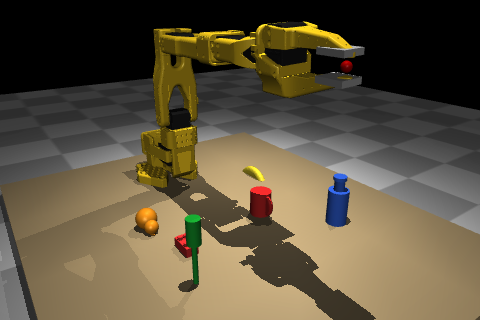
\includegraphics[width=0.18\textwidth]{figures/film_so101_reach_0.png} &
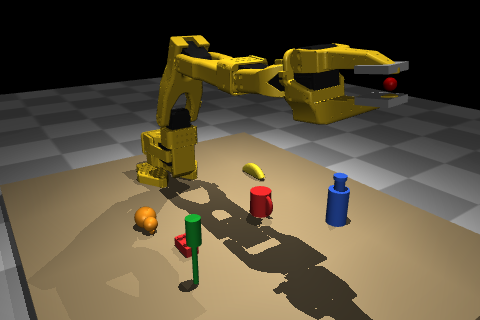
\includegraphics[width=0.18\textwidth]{figures/film_so101_reach_1.png} &
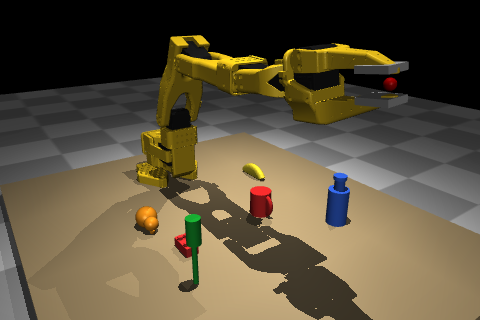
\includegraphics[width=0.18\textwidth]{figures/film_so101_reach_2.png} &
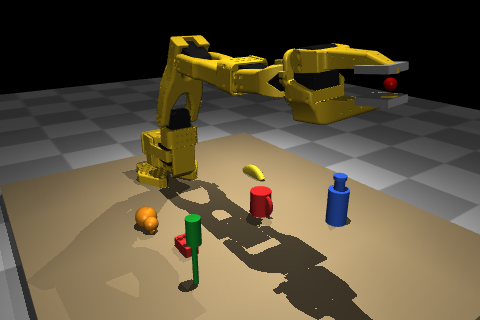
\includegraphics[width=0.18\textwidth]{figures/film_so101_reach_3.png} &
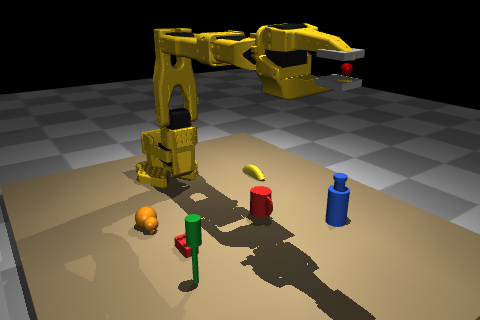
\includegraphics[width=0.18\textwidth]{figures/film_so101_reach_4.png} \\
\multicolumn{5}{c}{\parbox{0.92\textwidth}{\small\textbf{(a) SO-101 \texttt{reach\_x+5}.}
Home $\rightarrow$ 33\% $\rightarrow$ 66\% $\rightarrow$ at target $\rightarrow$ return-to-home.
$N{=}10$ trials, 10/10 pass (\S\ref{sec:cap-cross}, Table~\ref{tab:cross-skill}).}} \\[6pt]

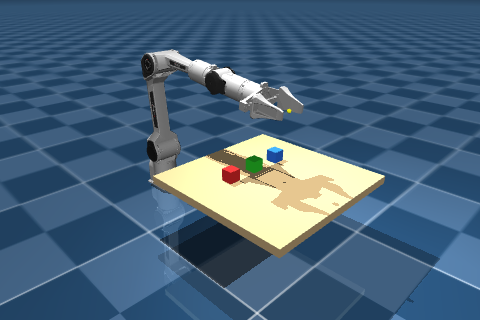
\includegraphics[width=0.18\textwidth]{figures/film_piper_pick_0.png} &
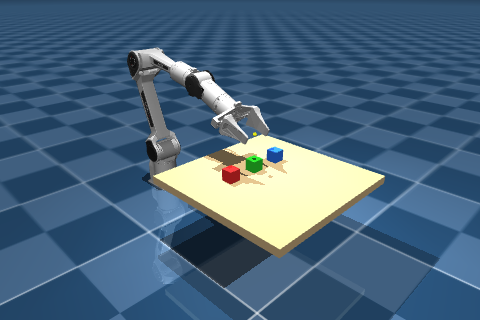
\includegraphics[width=0.18\textwidth]{figures/film_piper_pick_1.png} &
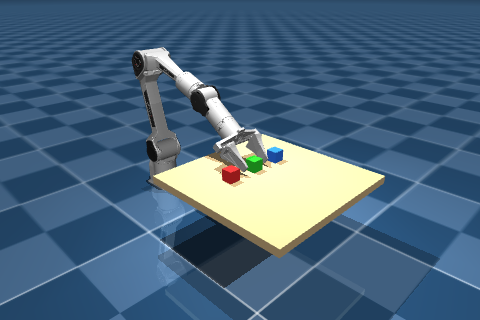
\includegraphics[width=0.18\textwidth]{figures/film_piper_pick_2.png} &
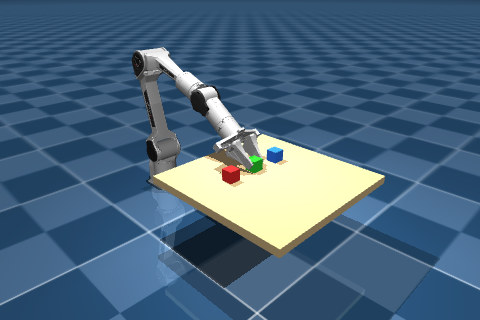
\includegraphics[width=0.18\textwidth]{figures/film_piper_pick_3.png} &
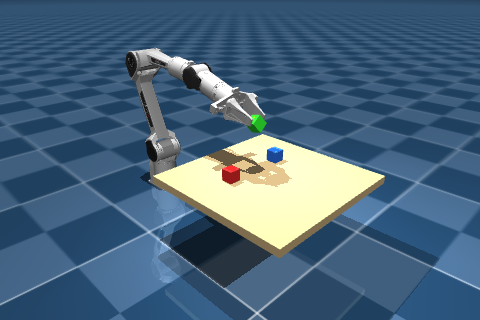
\includegraphics[width=0.18\textwidth]{figures/film_piper_pick_4.png} \\
\multicolumn{5}{c}{\parbox{0.92\textwidth}{\small\textbf{(b) Piper \texttt{pick\_green}.}
Home (gripper open) $\rightarrow$ 8\,cm pre-grasp $\rightarrow$
lower to the cube $\rightarrow$ \texttt{gripper\_close} (weld to cube)
$\rightarrow$ lift 12\,cm. The agent-written \texttt{gripper\_close}
does the distance check and weld activation; the 13-line
post-synthesis patch adds \texttt{get\_object\_position} and the
weld relpose update (\S\ref{sec:cap-cross-robot}).}} \\[6pt]

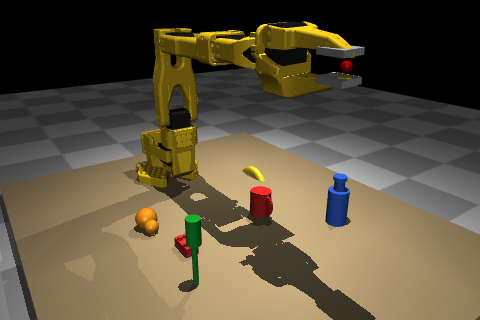
\includegraphics[width=0.18\textwidth]{figures/film_so101_letter_0.png} &
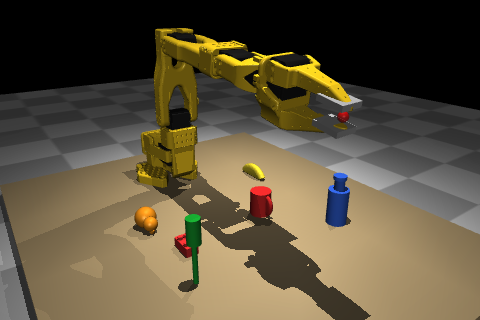
\includegraphics[width=0.18\textwidth]{figures/film_so101_letter_1.png} &
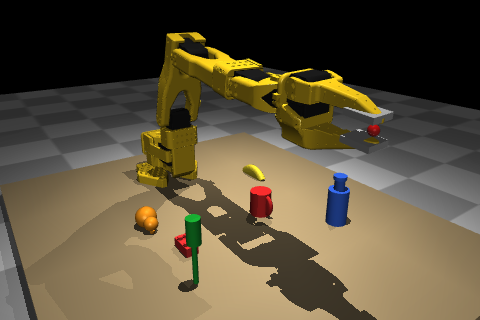
\includegraphics[width=0.18\textwidth]{figures/film_so101_letter_2.png} &
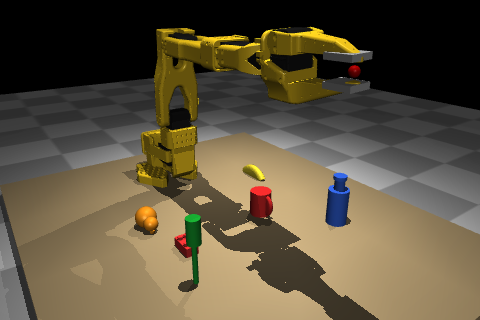
\includegraphics[width=0.18\textwidth]{figures/film_so101_letter_3.png} &
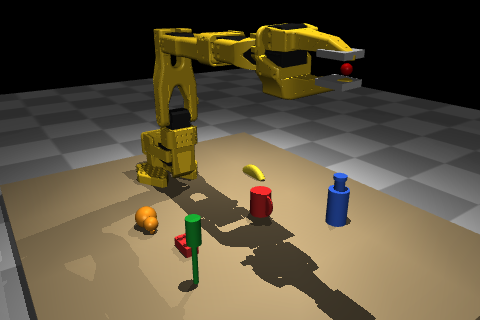
\includegraphics[width=0.18\textwidth]{figures/film_so101_letter_4.png} \\
\multicolumn{5}{c}{\parbox{0.92\textwidth}{\small\textbf{(c) SO-101 \texttt{draw\_letter\_L}}
(hard suite; graded trajectory re-executed by the synthesized driver). A two-leg L within the
SO-101 workspace: 4\,cm down, then 4\,cm forward ($+X$), then return
home. Graded by \texttt{ee\_waypoint\_trace}, which verifies the
end-effector actually visits both corners (in order) and returns
home, not merely the return. $N{=}5$ per model,
\S\ref{sec:cap-portability}.}} \\[6pt]

\multicolumn{1}{c}{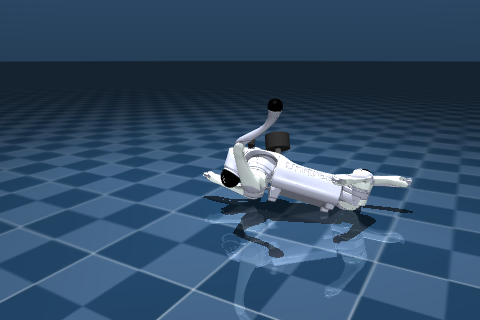
\includegraphics[width=0.18\textwidth]{figures/film_go2_walk_0.png}} &
\multicolumn{1}{c}{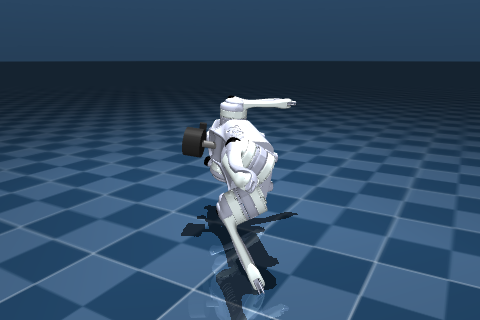
\includegraphics[width=0.18\textwidth]{figures/film_go2_walk_1.png}} &
\multicolumn{1}{c}{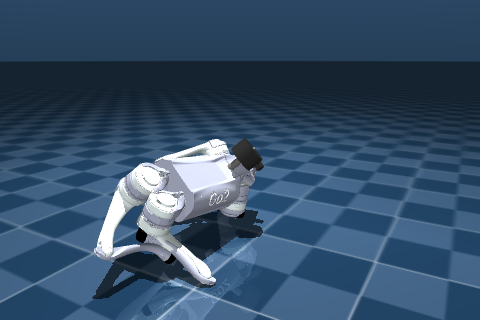
\includegraphics[width=0.18\textwidth]{figures/film_go2_walk_2.png}} &
\multicolumn{1}{c}{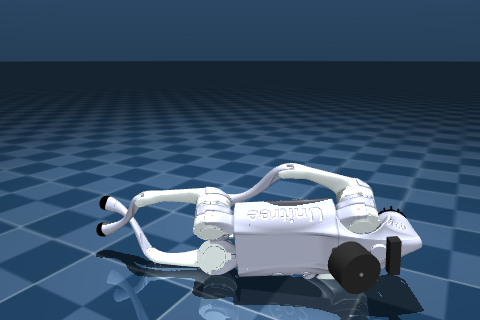
\includegraphics[width=0.18\textwidth]{figures/film_go2_walk_3.png}} &
\multicolumn{1}{c}{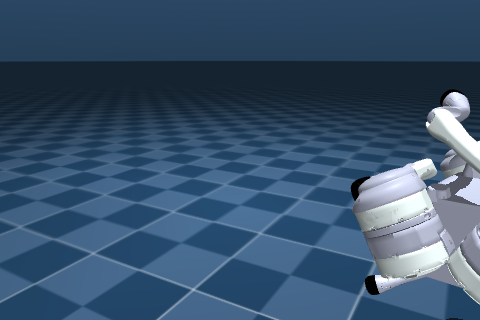
\includegraphics[width=0.18\textwidth]{figures/film_go2_walk_4.png}} \\
\multicolumn{5}{c}{\parbox{0.92\textwidth}{\small\textbf{(d) Go2 \texttt{sit} $\rightarrow$ \texttt{stand\_up} attempt}
(driver primitives executed live). The visible instability is the
point: the driver passes the 8/8 onboarding validation
(Table~\ref{tab:onboarding-detail}), yet the independent smoke
suite scores \texttt{stand\_up} 0/2 (Appendix~\ref{app:smoke}): the
validator-leniency gap disclosed in Appendix~\ref{app:onboarding},
and the reason every \S\ref{sec:capability} number is graded by
independent physics, never by the onboarding harness.}} \\
\end{tabular}
\caption{Task-execution filmstrips (manipulation and Go2). Five
frames per row, captured at evenly-spaced time points during a
single rollout of the agent-synthesized driver. Underlying
simulator is MuJoCo (\S\ref{sec:protocol}). All frames are
produced from the same artifacts that drive the quantitative
results in the body of the paper.}
\label{fig:filmstrips}
\end{figure*}

\begin{figure*}[t]
\centering
\setlength{\tabcolsep}{1pt}
\renewcommand{\arraystretch}{0.3}
\begin{tabular}{ccccc}
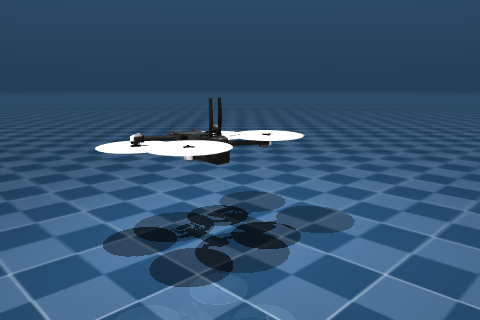
\includegraphics[width=0.18\textwidth]{figures/film_skydio_0.png} &
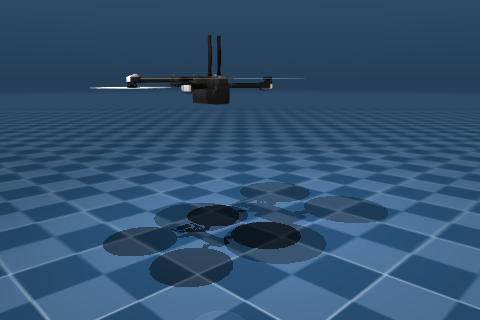
\includegraphics[width=0.18\textwidth]{figures/film_skydio_1.png} &
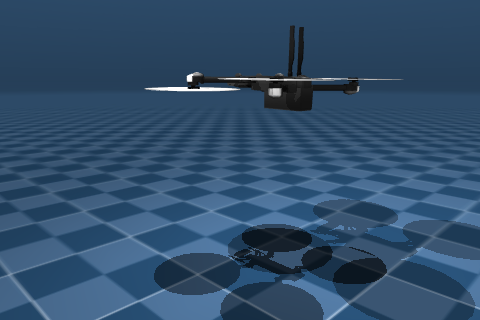
\includegraphics[width=0.18\textwidth]{figures/film_skydio_2.png} &
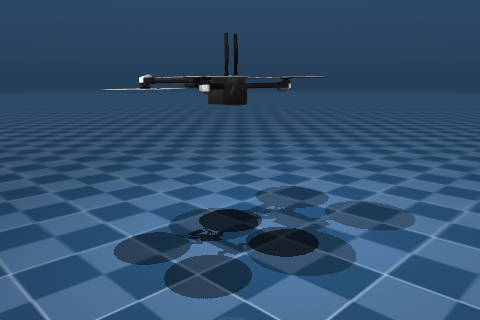
\includegraphics[width=0.18\textwidth]{figures/film_skydio_3.png} &
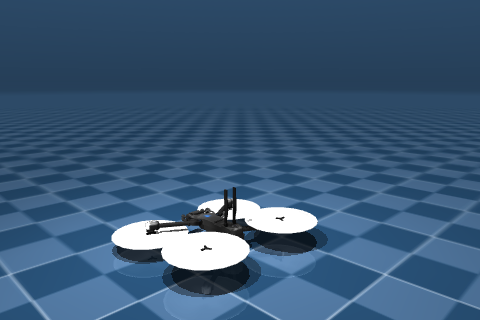
\includegraphics[width=0.18\textwidth]{figures/film_skydio_4.png} \\
\multicolumn{5}{c}{\parbox{0.92\textwidth}{\small\textbf{(e) Skydio~X2 quadrotor go-to}
(aerial suite, Appendix~\ref{app:morphology}). Ground $\rightarrow$
\texttt{takeoff} to 0.5\,m $\rightarrow$ \texttt{move\_to}
$(0.4, 0, 0.5)$ $\rightarrow$ return $\rightarrow$ \texttt{land}.
The cascaded position$\rightarrow$attitude$\rightarrow$thrust
controller is synthesized zero-shot from the MJCF; both agent
styles score $8/8$ on the hardened aerial suite
(Table~\ref{tab:aerial}).}} \\[6pt]

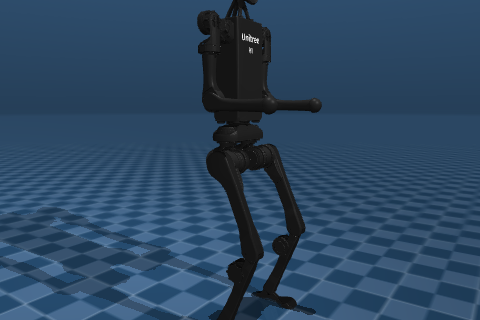
\includegraphics[width=0.18\textwidth]{figures/film_h1_0.png} &
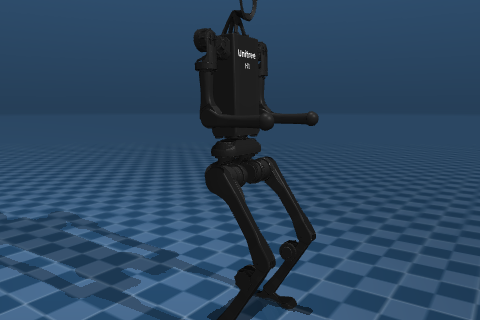
\includegraphics[width=0.18\textwidth]{figures/film_h1_1.png} &
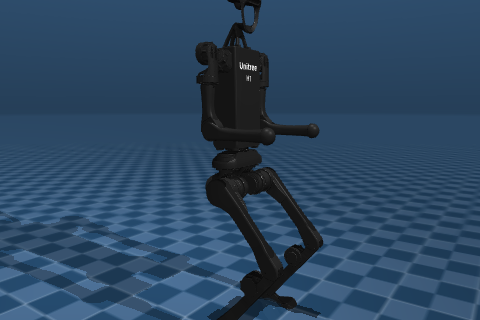
\includegraphics[width=0.18\textwidth]{figures/film_h1_2.png} &
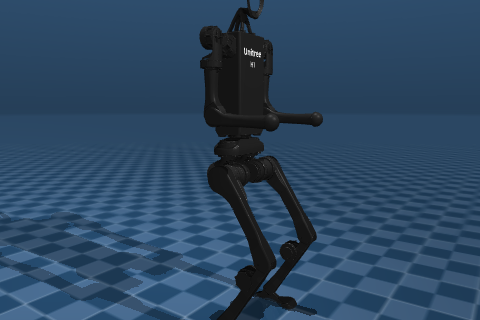
\includegraphics[width=0.18\textwidth]{figures/film_h1_3.png} &
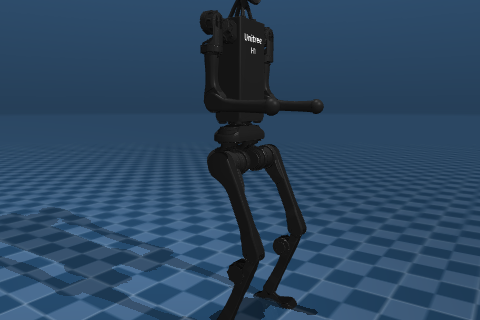
\includegraphics[width=0.18\textwidth]{figures/film_h1_4.png} \\
\multicolumn{5}{c}{\parbox{0.92\textwidth}{\small\textbf{(f) H1 humanoid squat-recover}
(Appendix~\ref{app:morphology}). The 19-DoF biped holds a PD-balanced
stand, bends at the knees and hips, and recovers without falling over;
the motion is deliberately conservative (torso dips from
0.98\,m and returns to 0.97\,m), which is what the validated
\texttt{squat} primitive does; dynamic walking remains the
pipeline's hardest open case (Appendix~\ref{app:morphology}).}} \\[6pt]

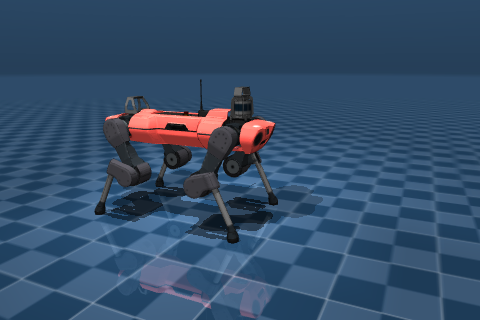
\includegraphics[width=0.18\textwidth]{figures/film_anymal_0.png} &
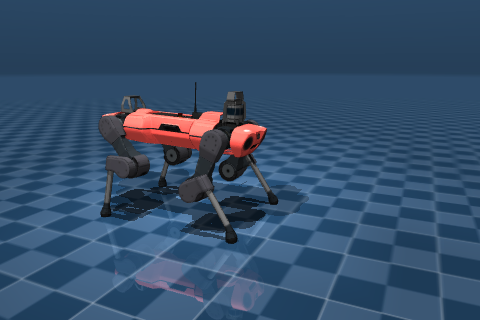
\includegraphics[width=0.18\textwidth]{figures/film_anymal_1.png} &
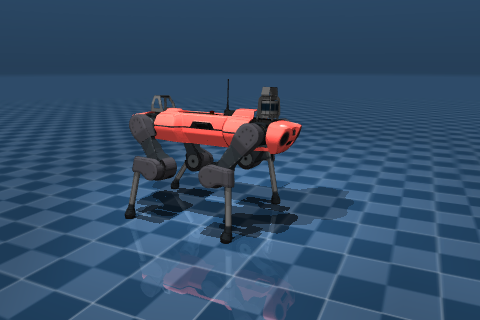
\includegraphics[width=0.18\textwidth]{figures/film_anymal_2.png} &
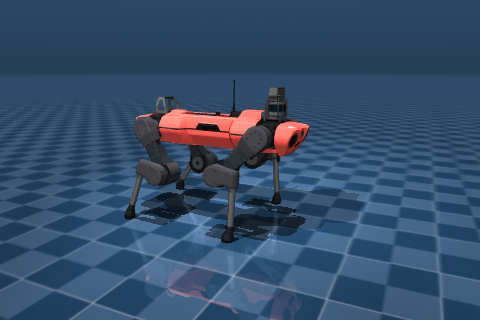
\includegraphics[width=0.18\textwidth]{figures/film_anymal_3.png} &
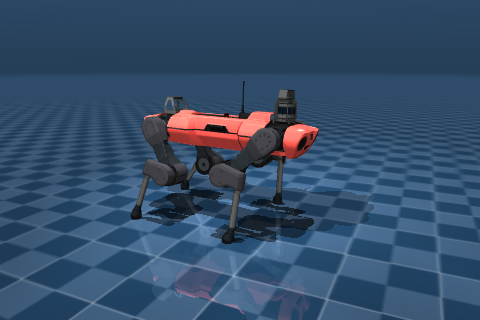
\includegraphics[width=0.18\textwidth]{figures/film_anymal_4.png} \\
\multicolumn{5}{c}{\parbox{0.92\textwidth}{\small\textbf{(g) ANYmal-C \texttt{walk\_forward}}
(locomotion v2 suite, \S\ref{sec:cap-cross-robot}). Stand, then four
2\,s \texttt{walk\_forward} calls at speed 0.2, the same call
pattern as the graded eval trials; the base advances 0.24\,m while
holding ${\approx}0.5$\,m body height. Executed live on the shared
driver behind the \S\ref{sec:cap-cross-robot} locomotion
comparison, where ANYmal-C favors Auto-Adapter (68\% vs.\ 28\%).}} \\
\end{tabular}
\caption{Morphology-breadth filmstrips (aerial, humanoid,
quadruped walking), rendered as in Figure~\ref{fig:filmstrips}.}
\label{fig:filmstrips2}
\end{figure*}
